O aprendizado supervisionado é o campo dentro de aprendizado de máquina que visa a gerar modelos preditores a partir de um conjunto de dados de treinamento cujos resultados são previamente conhecidos.

\section{Naive Bayes}

\textit{Naive Bayes} é uma das técnicas mais simples disponíveis nesse contexto. Ela se baseia no teorema de Bayes enquanto assume independência entre as características escolhidas para descrever o dado. Abaixo veremos sua formulação matemática como descrita por Schütze \cite{schutze08}.

Tendo $\mathbf{x}$ tal que $\mathbf{x} \in \mathbf{X}$ em que $\mathbf{X}$ é o conjunto de dados de treinamento, a sua probabilidade de pertencer a classe $c_k \in \mathbf{c}$ é dada pelo teorema de Bayes:
\begin{equation} \label{eq:bayes}
    p(c_k \mid \mathbf{x}) = \frac{p(c_k) \ p(\mathbf{x} \mid c_k)}{p(\mathbf{x})}
\end{equation}

Sendo $\mathbf{x}$ um vetor de $n$ características, ao se assumir independência entre elas obtém-se:
\begin{equation}
    p(x_i \mid x_{i+1}, \dots ,x_{n}, c_k ) = p(x_i \mid c_k)
\end{equation}

Logo, pode-se rescrever a equação \ref{eq:bayes} substituindo $p(\mathbf{x} \mid c_k)$ pelo produtório de suas características:
\begin{equation}
    p(c_k \mid \mathbf{x}) = \frac{p(c_k) \prod_{i=1}^n p(x_i \mid c_k)}{p(\mathbf{x})}
\end{equation}

Como $p(\mathbf{x})$ será uma constante dado cada exemplo $\mathbf{x}$ esta pode ser desprezada:
\begin{equation}
    p(c_k \mid \mathbf{x}) \propto p(c_k) \prod_{i=1}^n p(x_i \mid c_k)
\end{equation}

Portanto, tem-se que o estimador ótimo $\hat{y}$ escolherá pela classe que atinja maior probabilidade:
\begin{equation}
    \hat{y} = \underset{k \in \{1, \dots, K\}}{\operatorname{max}} \ p(c_k) \displaystyle\prod_{i=1}^n p(x_i \mid c_k)
\end{equation}

Vê-se então que o modelo de \textit{Naive Bayes} depende apenas de $p(c_k)$ e $p(\mathbf{x} \mid c_k)$. Estes parâmetros serão extraídos do conjunto de treino por máxima verosimilhança.

Dado um vetor $\mathbf{y}$ de tamanho $m$ que representa as classificações referentes a $\mathbf{X}$, pode-se estimar $p(c_k)$ pela contagem de vezes que a classe $c_k$ aparece no conjunto de treinamento:
\begin{equation}
    \hat{p}(c_k) = \frac{\sum_{i=1}^m [y_i = c_k]}{m}
\end{equation}

Por sua vez, $p(x_r \mid c_k)$ é estimado utilizando a contagem de vezes que uma característica aparece dividida pelo total de características presentes em $\mathbf{X'}$ que é o subconjunto de treino pertencente a classe $c_k$:
\begin{equation}
    \hat{p}(x_r \mid c_k) = \frac{\sum_{j=i}^{m'} \sum_{i=1}^n [x_{ji} = x_r]}{|\mathbf{X'}|}
\end{equation}

Vê-se que modelos montados a partir de \textit{Naive Bayes} são computacionalmente baratos dado que seus parâmetros são obtidos através de contagens sobre os dados de treinamento e que sua predição utiliza apenas multiplicações.
Embora se baseie na independência entre características, seu baixo custo operacional leva esta técnica a ser utilizada mesmo em problemas com notória dependência de características como a classificação de texto \cite{mccallum98}.

\section{SVM}

O conceito fundamental do \textit{Support Vector Machine} se dá pela obtenção de um vetor de suporte que melhor separe as classes. Esta separação é feita de maneira que se maximize a margem entre as classes. A figura \ref{fig:svm} demostra dados de duas classes distintas, representadas pelas cores rosa e amarelo, pertencentes a um espaço de características de duas dimensões; vê-se na figura que a reta que define a maior separação é suportada pelos dados de cada classe mais próximos a ela.

\begin{figure}
\begin{center} {
    \begin{center}
    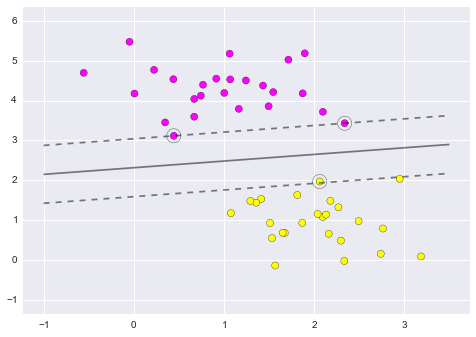
\includegraphics[scale=0.7]{svm.png}
    \caption{Reta de maior margem entre classes.}
    \small Imagem com direitos cedidos para uso não comercial, retirada de \cite{vanderplas15}
    \label{fig:svm}
    \end{center}
}
\end{center}
\end{figure}

Por se basear nos dados próximos ao limiar de separação das classes, o algoritmo passa a ser incapaz de distinguir os casos de classes que não são separáveis sem erros. A solução desse problema foi a criação de uma variável de relaxamento que define um número máximo de erros de classificação permitido. Esta propriedade é descrita com mais detalhes por Cortes e Vapnik em \cite{cortes95}. Sua utilização permite o desenvolvimento de modelos mais robustos a \textit{outliers} e melhora a generalização. Outros exemplos de regularizadores, como este, serão apresentados na subseção \ref{regularizadores}.

Como utilizam vetores de suporte para definir hiperplanos de separação, SVMs não são capazes de segregar classes não linearmente distinguiveis. Podemos observar um exemplo deste caso na figura \ref{fig:svm-lin}, na qual um SVM treinado tenta separar classes concêntricas.

\begin{figure}
\begin{center} {
    \begin{center}
    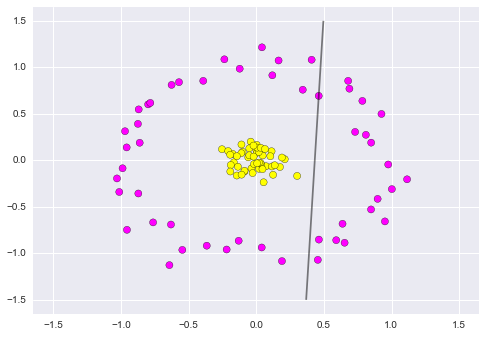
\includegraphics[scale=0.7]{svm-lin.png}
    \caption{SVM em dados não linearmente separáveis.}
    \small Imagem com direitos cedidos para uso não comercial, retirada de \cite{vanderplas15}
    \label{fig:svm-lin}
    \end{center}
}
\end{center}
\end{figure}

Para contornar esse impedimento, foi elaborado o que se chamou de \textit{kernel trick}. Este se baseia em um mapeamento não linear dos dados para um espaço onde possam ser linearmente separáveis \cite{scholkopf02}. A figura \ref{fig:svm-rbf} mostra a representação dos dados apresentados na figura \ref{fig:svm-lin} após seu mapeamento por uma função de base radial.

\begin{figure}
\begin{center} {
    \begin{center}
    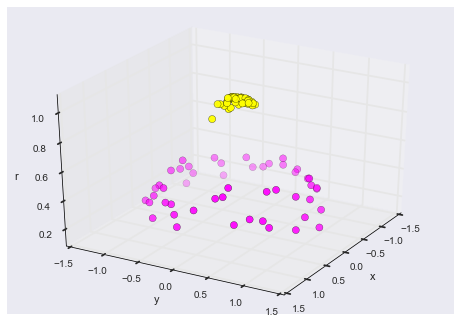
\includegraphics[scale=0.7]{svm-rbf.png}
    \caption{Transformação de dados por função de base radial.}
    \small Imagem com direitos cedidos para uso não comercial, retirada de \cite{vanderplas15}
    \label{fig:svm-rbf}
    \end{center}
}
\end{center}
\end{figure}

Neste novo espaço definido pela transformação, os dados são linearmente separáveis. Portanto, é possível achar um vetor de suporte que defina um hiperplano de separação das classes. Vemos na figura \ref{fig:svm-rbf-clas} as margens encontradas.

\begin{figure}
\begin{center} {
    \begin{center}
    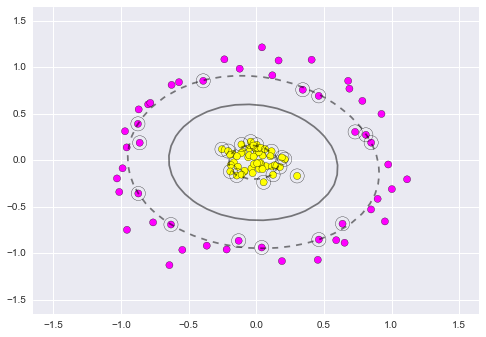
\includegraphics[scale=0.7]{svm-rbf-clas.png}
    \caption{SVM com \textit{kernel} de base radial.}
    \small Imagem com direitos cedidos para uso não comercial, retirada de \cite{vanderplas15}
    \label{fig:svm-rbf-clas}
    \end{center}
}
\end{center}
\end{figure}

Uma limitação na utilização deste algoritmo é seu tempo de treinamento. Sua complexidade computacional fica entre $O(n_{caracteristicas} \times n_{dados}^2)$ e $O(n_{caracteristicas} \times n_{dados}^3)$ \cite{list09}. Porém, Suykens e Vandewalle desenvolveram uma função custo através da qual tornou possível realizar o treinamento de SVMs a partir da otimização pelo método do gradiente \cite{suykens99}.

\section{Redes Neurais}

Redes Neurais são sistemas computacionais que visam replicam o modelo de processamento do cérebro. Há diversas variações de Redes Neurais, nesta seção abordaremos a mais simples, Redes Neurais FeedForward, apresentaremos Redes Neurais Convolucionais na subseção \ref{convolucionais}.

Redes Neurais FeedForward são compostas de camadas de neurônios interligados por sinapses. As sinapses funcionam como um ponderador linear dos neurônios da camada anterior. Os neurônios, por sua vez, representam uma função de ativação, normalmente não linear, tais como: tangente hiperbólica, \textit{sigmoid}, etc. Nesta categoria

Uma de suas principais características é a capacidade de aproximar qualquer função dado que a rede contenha pelo menos uma camada escondida com número suficientemente grande de neurônios com ativação não linear \cite{hornik89}.

backprop

\subsection{Deep Learning}

\subsection{Redes Neurais Convolucionais} \label{convolucionais}

\section{Regularizadores} \label{regularizadores}

\subsection{L2}

\subsection{Dropout}

\section{Otimizadores}

\subsection{Momentum}

\subsection{RMSProp}

\subsection{Adam}

\section{Supervisão Distante}
